\documentclass[12pt]{article}
\usepackage{mathtools}
\usepackage{graphicx}
\usepackage{float}

\setlength{\parindent}{0in}
\setlength{\parskip}{0ex}

\setlength{\textheight    }{9.0in}
\setlength{\textwidth     }{6.5in}
\setlength{\oddsidemargin }{0.0in}
\setlength{\evensidemargin}{0.0in}
\setlength{\headheight    }{-0.3in}
\setlength{\headsep       }{0.0in}
\setlength{\textheight    }{9.0in}

\begin{document}

\begin{center}
\Large{COSC 223: Probability and Computing} \\
\Large{Project 2: Queueing} \\ 
\large{Juhwan Jeong and Ian McClaugherty} \\
\large{April 13, 2019}
\end{center}

\section{Introduction}
In this project, we are studying how variability in job size and interarrival time affects mean response time on a single-server queueing system with a First Come First Serve Policy. Essentially, a queue is an ordered line. Queues are common in everyday life. For example, one often encountered queue is the checkout line in a grocery store. The checkout line happens to be an example of the First Come First Serve Policy that we are using in this project: the first person in the line is the first to get checked out. In other words, customers check out in the order in which they show up in line.  \\ 
Queueing is also common in computer science and has many important applications. Tasks like CPU scheduling, reading from a disk, and network routing all rely on queues. Two queue parameters that are crucial to consider are job size and interarrival time.  Job size is the amount of time that a job spends on a server when it is being processed. Interarrival time is the time that passes between two consecutive Understanding the factors that impact the performance of a queueing system allows us to better predict its performance, as long as we have some basic knowledge about the jobs which the queue is going to run. The goal of this project is to learn about how variability in job size (how long it takes to run a job on the server) and interarrival time (the time between job arrivals) changes the average amount of time that a job spends in the queuing system. 

\section{Experimental Setup}
In the first experiment, we simulated the queueing system for 1,000,000 jobs. The interarrival times were drawn from an exponential distribution with parameter $\lambda$, where $\lambda$ ranged from 0.01 to 1 with 0.01 increments. The job sizes were drawn from a hyperexponential distribution, where the variance was either 1, 10, 20, or 50. Given each variance, the following series of calculations was performed to acquire values of $\mu_1$, $\mu_2$, and $p$. \\
First, we compute $E[X]$, where $X$ is a random variable that represents job size. In class, we used integration by parts to show that the expected value of an exponential with rate $\lambda$ is $\frac{1}{\lambda}$. To compute the expected value of the hyperexponential, we first multiply the expected value of each exponential by its corresponding probability, then sum those products: 
\begin{align*} 
E[X] &= p \int_{0}^{\infty} x \mu_1 e^{-\mu_1 x} ~ dx + (1-p) \int_{0}^{\infty} x \mu_2 e^{-\mu_2 x} ~ dx \\
&= p(\frac{1}{\mu_1}) + (1-p)(\frac{1}{\mu_2}) \\
&= \frac{p}{\mu_1} + \frac{1-p}{\mu_2}
\end{align*}
Because we are assuming that $E[X] = 1$ and that $\frac{p}{\mu_1} = \frac{1-p}{\mu_2}$, we can compute the values for $\mu_1$ and $\mu_2$: 
\begin{align*}
E[X] &= \frac{p}{\mu_1} + \frac{1-p}{\mu_2} = 1 \\
&\Rightarrow
\frac{p}{\mu_1} = \frac{1-p}{\mu_2} = \frac{1}{2} \\
&\Rightarrow
\mu_1 = 2p, \mu_2 = 2(1-p)
\end{align*}
To compute $E[X^2]$, we evaluate the following integral: 
\begin{align*} 
E[X^2] = p \int_{0}^{\infty} x^2 \mu_1 e^{-\mu_1 x} ~ dx + (1-p) \int_{0}^{\infty} x^2 \mu_2 e^{-\mu_2 x} ~ dx
\end{align*}
Solving this integral requires using integration by parts, and the technique is very similar to the one we used in class to solve the integral for $E[X]$. Consider the following choices for $u$ and $dv$ for the first term in the sum (which uses rate $\mu_1$):
\begin{align*}
u &= x^2 \\
du &= 2x \: dx \\ 
dv &= \mu_1e^{-\mu_1 x} \\
v &= -e^{-\mu_1 x}
\end{align*}
Now, we can write the first term as follows:
\begin{align*}
&= p[-x^2e^{-\mu_1 x} \biggr\rvert_{x = 0}^{\infty} - \int_{0}^{\infty} -e^{-\mu_1 x} 2x ~ dx]
\end{align*}
We can turn this integral into the integral for $E[X]$ by rewriting the $2$ as $\frac{2\mu_1}{\mu_1}$ and then pulling $\frac{2}{\mu_1}$ out in front:
\begin{align*}
&= p[-x^2e^{-\mu_1 x} \biggr\rvert_{x = 0}^{\infty} + \frac{2}{\mu_1} \int_{0}^{\infty} x \mu_1 e^{-\mu_1 x} ~ dx]
\end{align*}
 As $x \rightarrow \infty$, the exponential grows much faster than $-x^2$, so $-x^2e^{-\mu_1 x} \biggr\rvert_{x = 0}^{\infty}$ evaluates to zero. We know the integral evaluates to $\frac{1}{\mu_1}$. Now, we have
\begin{align*}
&= p[\frac{2}{\mu_1}(\frac{1}{\mu_1})] = \frac{2p}{\mu_1^2}
\end{align*}
We can perform the same steps for the second term in the expression for $E[X^2]$. The final result is below:
\begin{align*}
E[X^2] = \frac{2p}{\mu_1^2} + \frac{2(1-p)}{\mu_2^2}
\end{align*}
The values of our parameters $\mu_1$, $\mu_2$, and $p$ depend upon the variance. Using the variance equation, we found an expression for $p$ in terms of the variance. 
\begin{align*} 
Var[X] &= E[X^2] - (E[X])^2 \\
&= \frac{2p}{\mu_1^2} + \frac{2(1-p)}{\mu_2^2} - (1)^2 \\
\intertext{Substituting $\mu_1 = 2p$ and $\mu_2 = 2(1-p)$ yields:} \\
&= \frac{1}{2p} + \frac{1}{2(1-p)} - 1 \\ 
&= \frac{1}{2p(1-p)} - 1
\end{align*}
Let $Var[X] = v$. We will solve for $p$ in terms of $v$. 
\begin{align*} 
&v = \frac{1}{2p(1-p)} - 1 \\
&v[2p(1-p)] = 1 - 2p(1-p) \\ 
&2p(1-p) + 2vp(1-p) - 1 = 0 \\ 
&2p - 2p^2 + 2vp - 2vp^2 - 1 = 0 \\
&p^2(-2 - 2v) + p(2v + 2) - 1 = 0 \\ 
&p^2(-2 - 2v) - p(-2 - 2v) - 1 = 0 \\ 
&p^2 - p + \frac{1}{2 + 2v} = 0 \\ 
\intertext{Using the quadratic formula, we get:} \\
&p = \frac{-(-1) \pm \sqrt{(-1)^2 + \frac{4}{2+2v}}}{2} \\
&p = \frac{1 \pm \sqrt{1 + \frac{2}{1+v}}}{2}
\end{align*}

We simulated the queueing system for each possible pair of $\lambda$ and variance values and recorded the mean response time. The results were graphed on a mean response time vs. $\lambda$ graph. \\

In the second experiment, we simulated the queueing system for 1,000,000 jobs again; this time, the interarrival times were drawn from a hyperexponential distribution with balanced means and the job sizes were drawn from an exponential distribution with $\lambda$ = 1. For the hyperexponential distribution, the expected value ranged from 1.01 to 4.00, with 0.01 increments (Note the expected values of interarrival times are at least 1, which is the expected value of job sizes, as we study the case where processing rate is strictly greater than the arrival rate). For each expected value $\mu$, the variance was set to be either $\mu$, $10\mu^2$, $20\mu^2$, $50\mu^2$. These variance values were used to ensure that the ratio between $\mu$ and $\sigma$ remained at 1, $\sqrt{10}$, $\sqrt{20}$, and $\sqrt{50}$ to accommodate for the fact that the mean is changing. Given each mean and variance, the following series of calculations were performed to acquire values of $\mu_1$, $\mu_2$, and $p$. \\

The calculations are similar to those above for experiment 1, the key difference being that $E[X]$, the expected value of interarrival times, is not fixed at 1. We let
\begin{align*}
E[X] = \frac{p}{\mu_1} + \frac{1-p}{\mu_2} = l
\end{align*}
where $l$ represents the expected value. Because our hyperexponential still has balanced means, 
\begin{align*}
&\frac{p}{\mu_1} = \frac{1-p}{\mu_2} = \frac{l}{2} \\
&\Rightarrow \mu_1 = \frac{2p}{l}, \mu_2 = \frac{2(1-p)}{l}
\end{align*}
These values help us solve for $E[X^2]$ in terms of $l$ and $p$: 
\begin{align*}
E[X^2] &= \frac{2p}{\mu_1^2} + \frac{2(1-p)}{\mu_2^2} \\
&= \frac{2pl^2}{4p^2} + \frac{2(1-p)l^2}{4(1-p)^2} \\ 
&= l^2(\frac{1}{2p} + \frac{1}{2(1-p)}) \\
&= \frac{l^2}{2p(1-p)}
\end{align*}
Now, we can solve for $p$ in terms of the variance $v$ and expected value $l$: 
\begin{align*}
&Var[X] = v = E[X^2] - (E[X])^2 \\
&v = \frac{l^2}{2p(1-p)} - l^2 \\
&2pv(1-p) = l^2 - 2pl^2(1-p) \\ 
&2pv - 2p^2v + 2pl^2 - 2p^2l^2 - l^2 = 0 \\ 
&p^2(-2v - 2l^2) - p(-2v - 2l^2) - l^2 = 0 \\ 
&p^2 - p + \frac{l^2}{2v + 2l^2} = 0 \\ 
&p = \frac{1 \pm \sqrt{1 + \frac{4l^2}{2v + 2l^2}}}{2}
\end{align*}

Again, we simulated the queueing system for each pair of $\lambda$ and variance values and recorded the mean response time. The results were graphed on a mean response time vs. $\lambda$ graph. 

\section{Results and Discussion} 
In experiment 1, we compute $\lambda$ and $\mu$ as the equivalent of arrival rate and processing rate, respectively. Using these quantities, we were able to make predictions on what the result might look like. The following two equations were used to draw a relationship between $E[T]$ and $\lambda$. First,

\begin{align*}
E[N] = \frac{\rho}{1 - \rho} = \frac{\frac{\lambda}{\mu}}{1 - \frac{\lambda}{\mu}} = \frac{\lambda}{\mu - \lambda} = \frac{\lambda}{1 - \lambda}
\end{align*}
since $\mu = 1$. Then, from Little's Law, we have 
\begin{align*}
&E[N] = \frac{\lambda}{1 - \lambda} = \lambda E[T] \\ 
&\Rightarrow 
E[T] = \frac{1}{1 - \lambda}
\end{align*}
As depicted in the relationship above, we expect the mean response time to increase as $\lambda$ increases from 0 to 1. \\

In experiment 2, we compute mean response time for each pair of expected value and variance of interarrival times. As expected value increases, the rate at which jobs arrive decreases. In turn, jobs will not get queued up as much, and mean response time will decrease. Therefore, we predict that as expected value of interarrival times increases, the mean response time will decrease. \\

As for variance, high variance will lead to higher chance of generating a value significantly lower or greater than the expected value. \\

In experiment 1, we generate service times from the same distribution with varying variances. When we have a distribution with a high variance, generating significantly shorter jobs will not have a great effect on the mean response time - the jobs will be processed quickly and it will not lead to longer queues. Generating longer jobs than usual, however, will significantly impact the mean response time since longer jobs can lead to longer queues, increasing the response time not only of the job itself, but also of the jobs that are to follow. Therefore, generating service times with higher variance will lead to greater mean response time. \\ 

In experiment 2, we generate interarrival times from the same distribution with varying variances. Opposite to experiment 1, when we have a distribution with a high variance, generating significantly longer interarrival time will not have a great effect on the mean response time - since jobs are less likely to get queued up with long interarrival times. Generating shorter jobs than usual, however, will significantly impact the mean response time since shorter interarrival times will lead to jobs getting queued up - elongating response times of multiple jobs. Therefore, generating interarrival times with higher variance will also lead to greater mean response time. \\ 

\pagebreak
The results of experiment 1 are as follows: 
\begin{figure}[H]
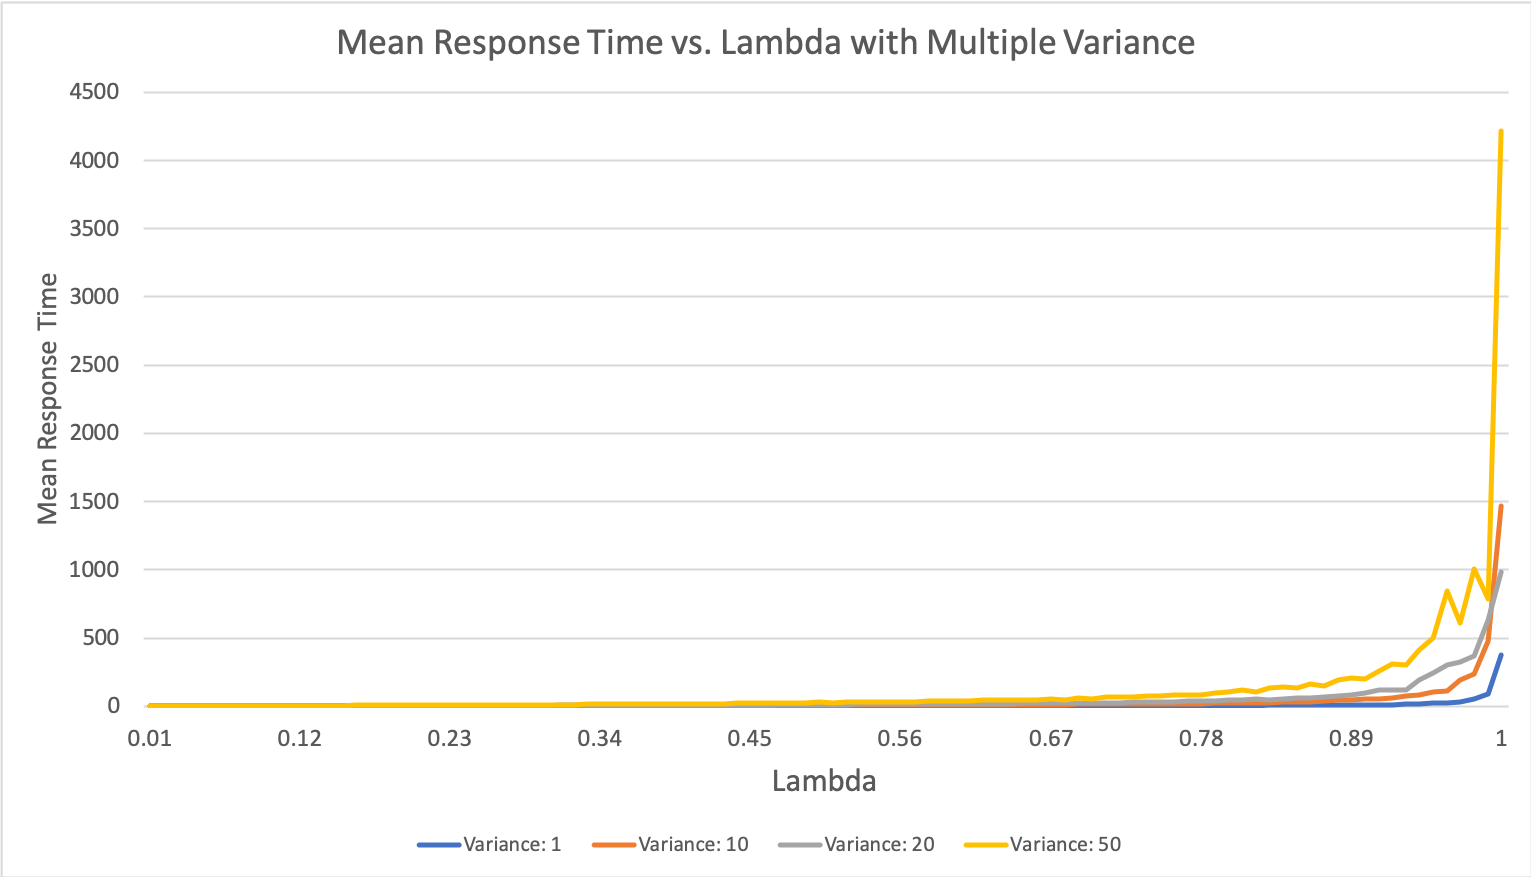
\includegraphics[ scale = 0.6]{Analysis.png}
\caption{Graph of Mean Response Time vs. $\lambda$ from Experiment 1 from $\lambda$ = 0 to 1, where $\lambda$ is the rate of the interarrival times distribution.}
\end{figure}

\begin{figure}[H]
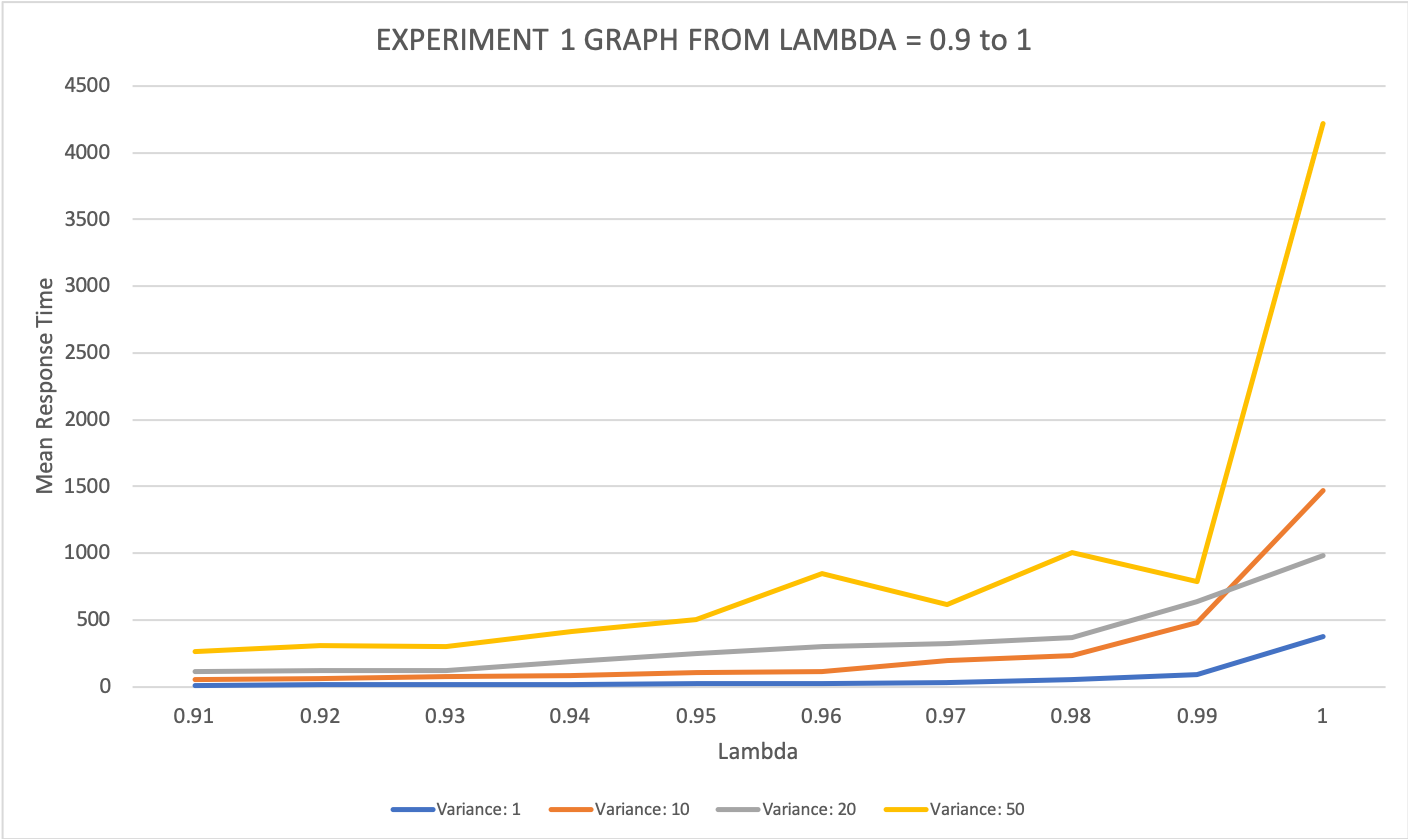
\includegraphics[scale = 0.6]{Graph1ZoomedIn.png}
\caption{Graph of Mean Response Time vs. $\lambda$ from Experiment 1 from $\lambda$ = 0.9 to 1, where $\lambda$ is the rate of the interarrival times distribution.}
\end{figure}
\pagebreak
In experiment 1, the graphs showed behaviors we expected. The curves had similar shape to $E[T] = \frac{1}{1-\lambda}$ and the mean response time increased as $\lambda$ increased, more specifically, as $\lambda$ approached 1 - the processing rate. This is because as interarrival times approach job sizes, jobs start to get queued up, and the mean response time increases. In addition, graphs with higher variances had higher mean response times as expected. This is due to the fact that with higher variance, the system is more likely to encounter a long service time, which leads to jobs getting queued up, lengthening response times of multiple jobs. \\

\begin{figure}[H]
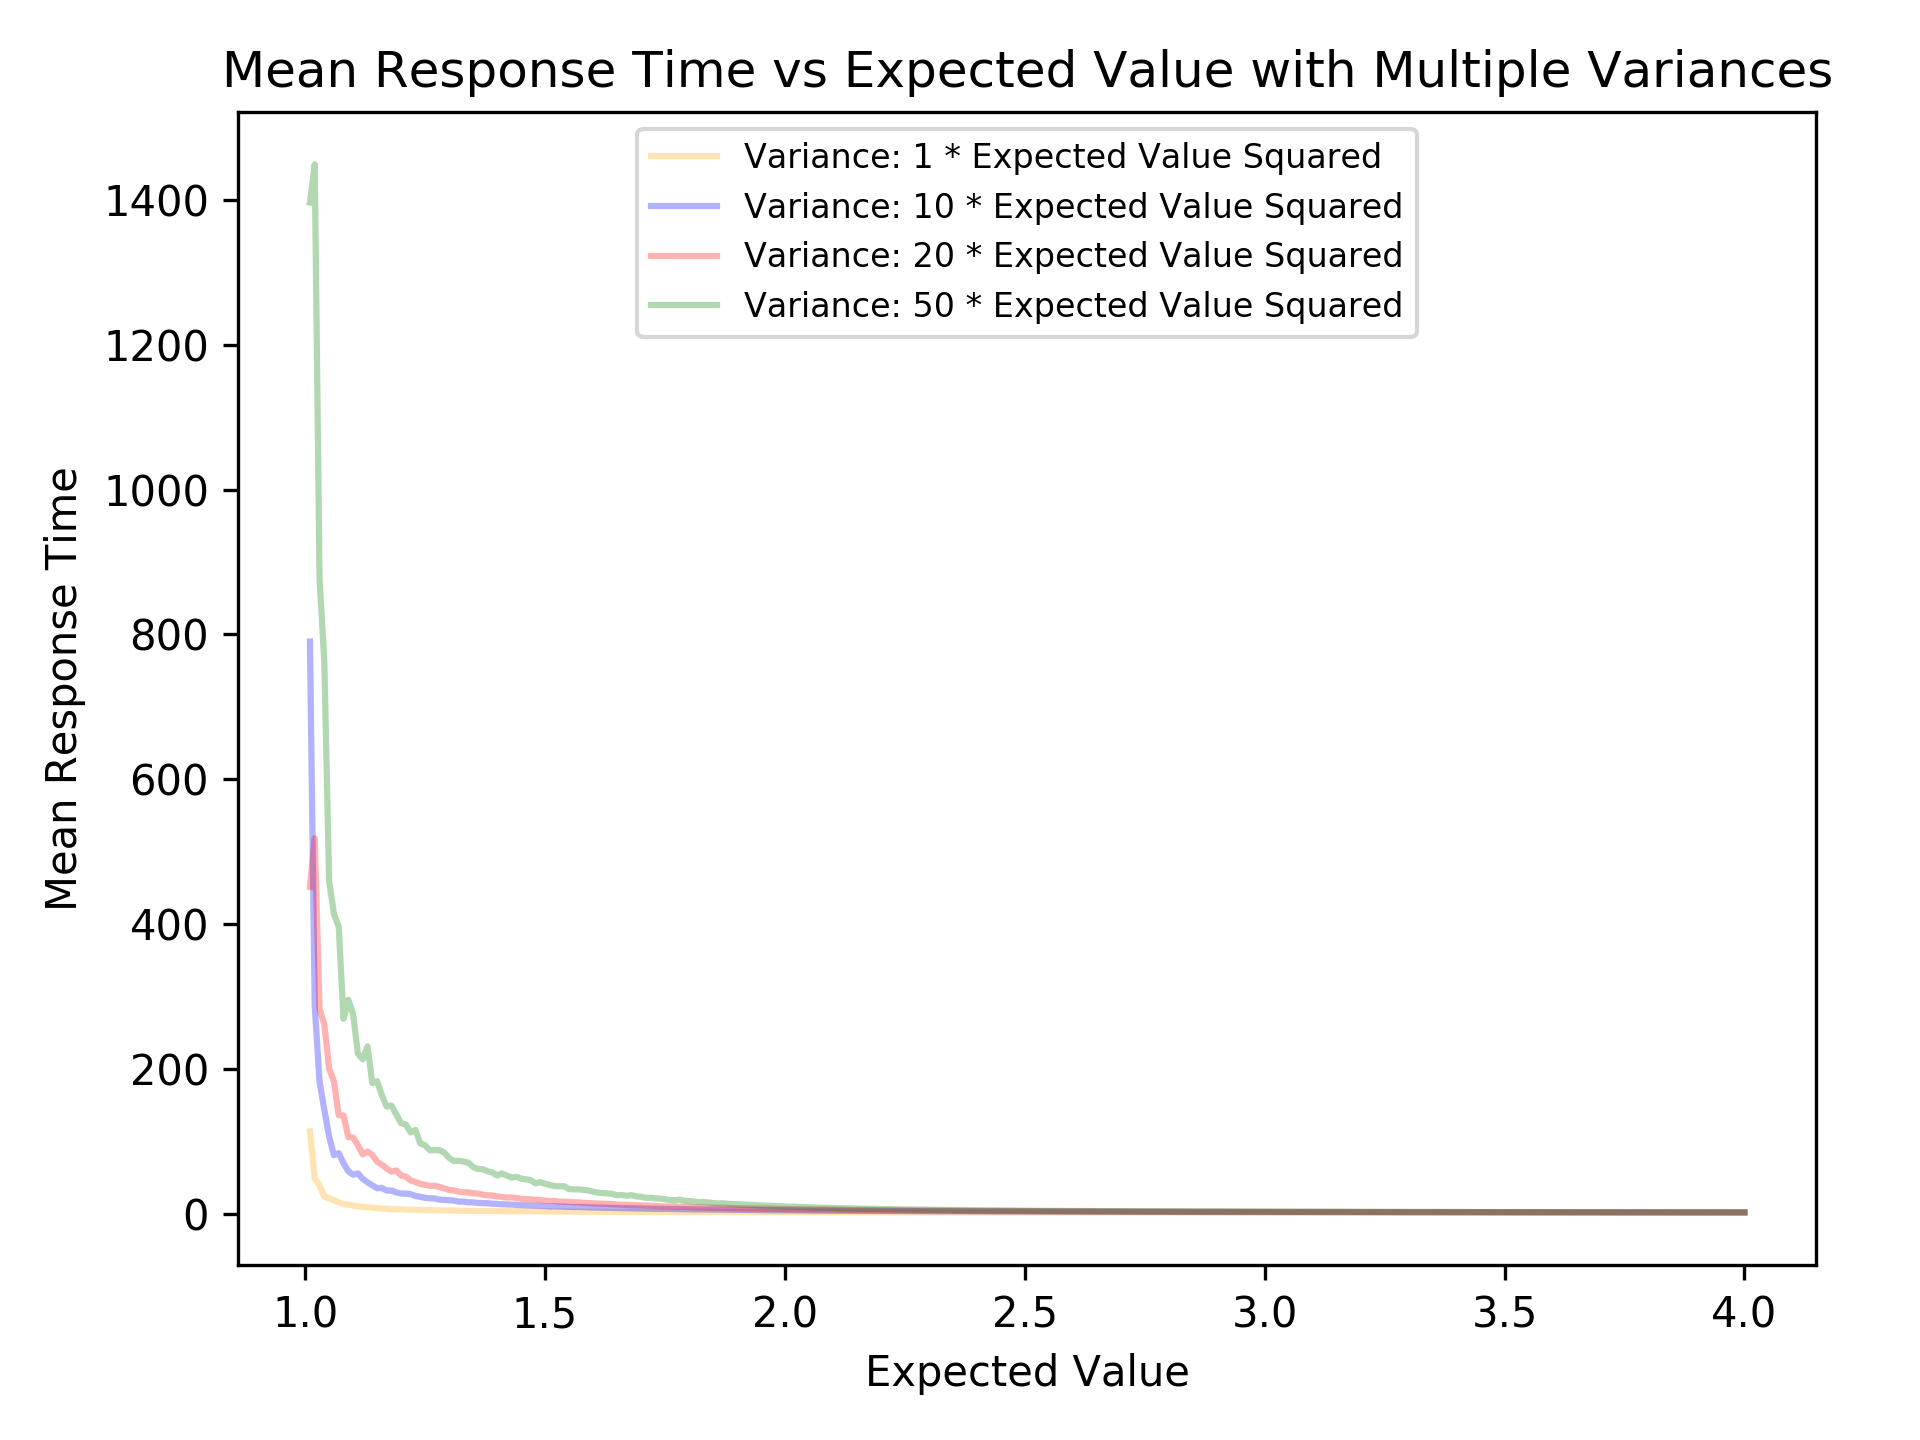
\includegraphics[width=\linewidth]{Analysis2_1.png}
\caption{Graph of Mean Response Time vs. Expected Value for Expected Values between 1.0 and 4.0 from Experiment 2.}
\end{figure}

\begin{figure}[H]
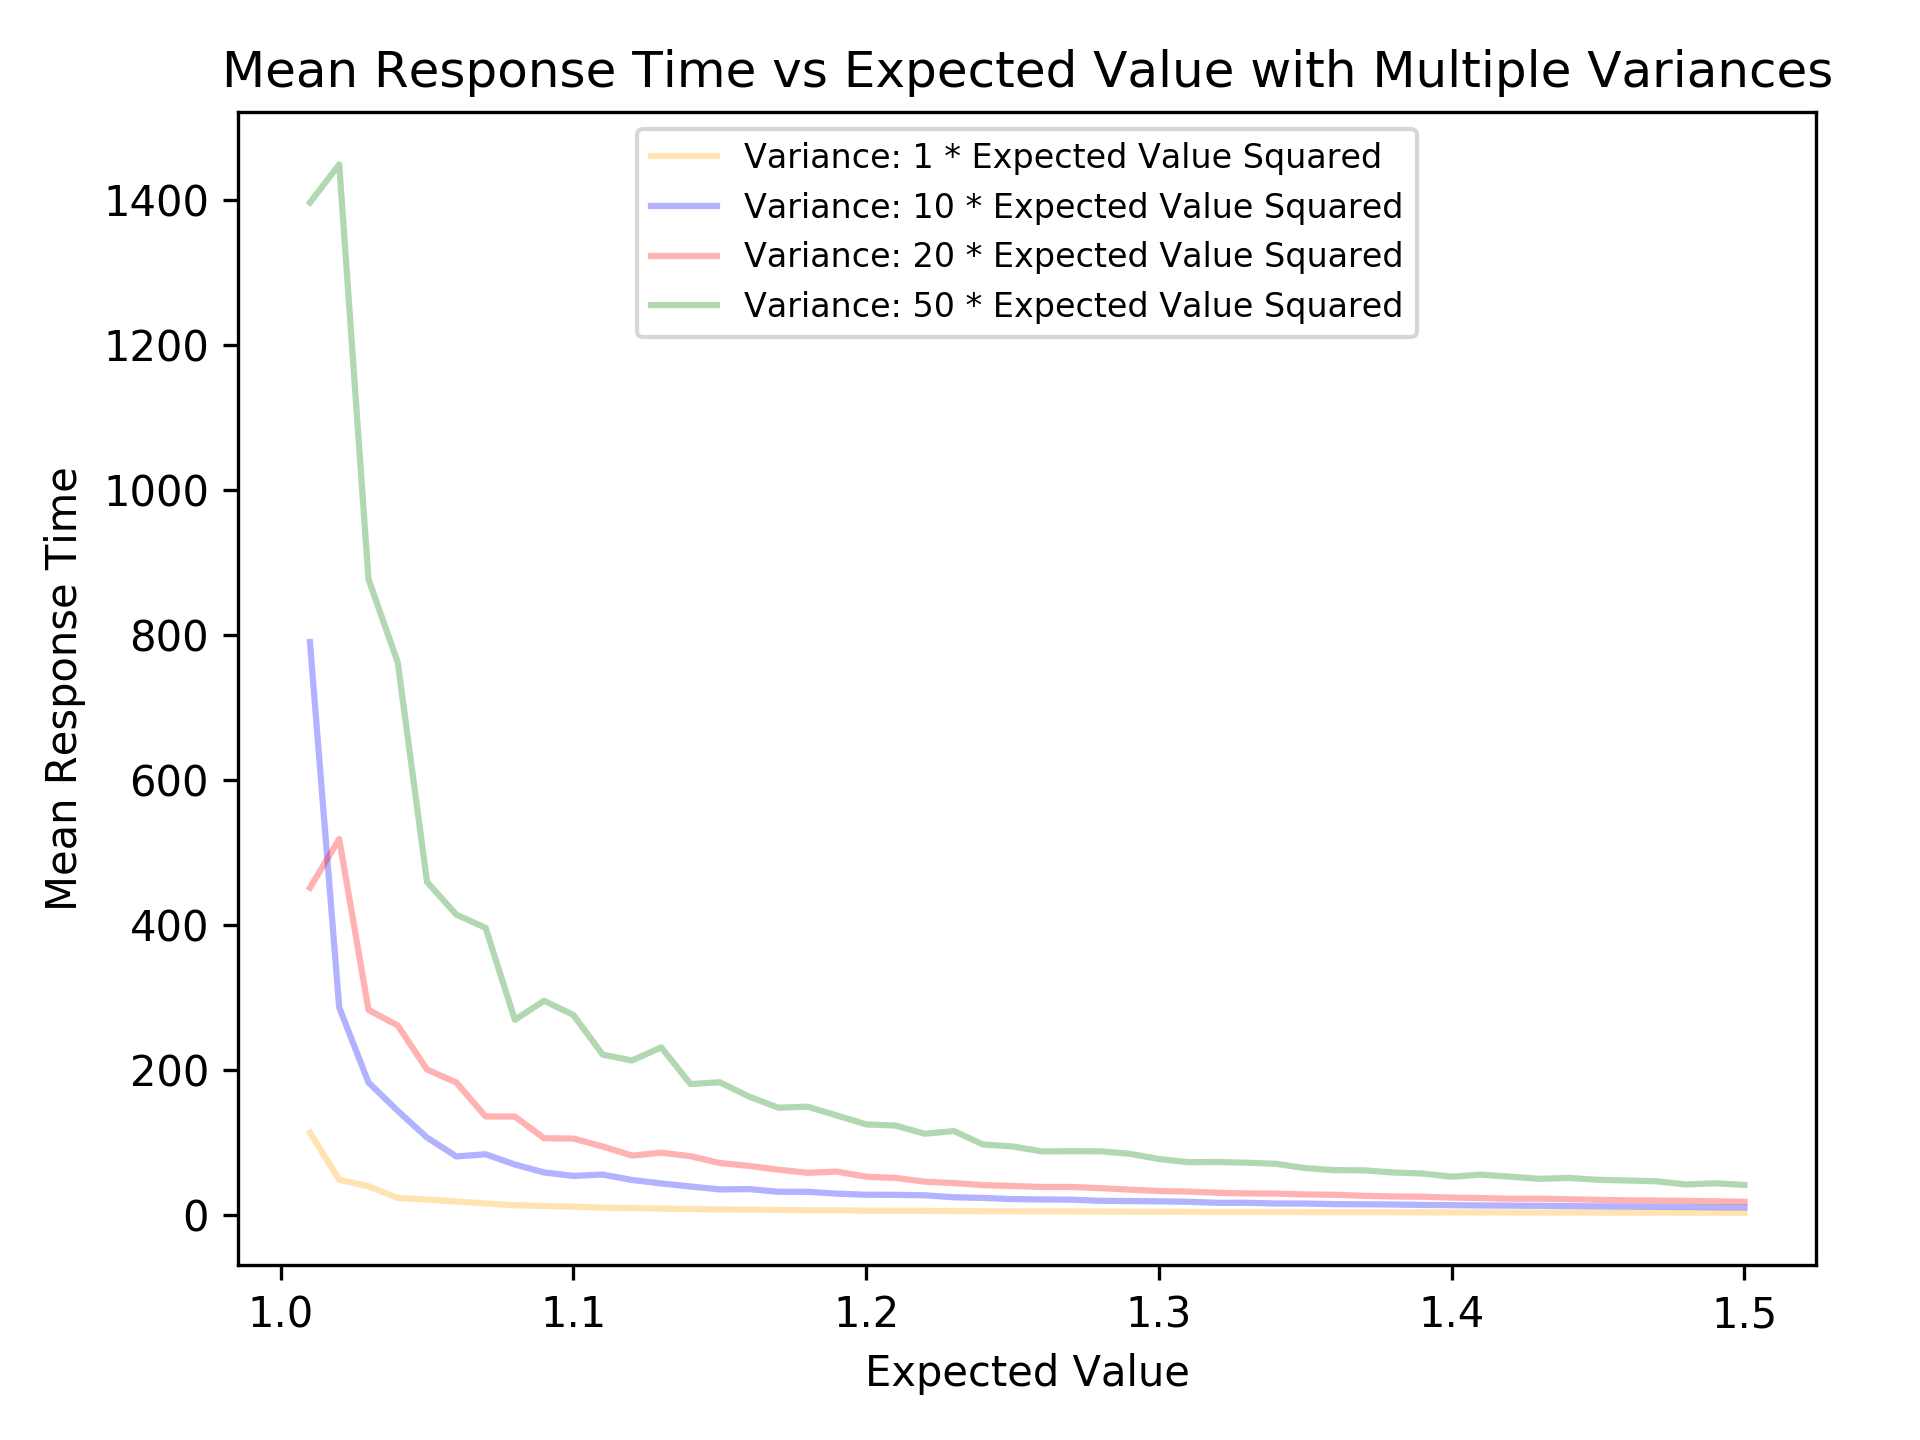
\includegraphics[width=\linewidth]{Analysis2_1_1.png}
\caption{Graph of Mean Response Time vs. Expected Value for Expected Values between 1.0 and 1.5 from Experiment 2.}
\end{figure}

In experiment 2, the graph exhibits behavior as predicted; as expected value of interarrival times increases, the mean response time decreases. When the interarrival times are comparable in length to service times, jobs are more likely to get queued up, which increases the mean response time. As interarrival times get longer, however, jobs get queued up less, and mean response time decreases drastically. In addition, graphs with higher variances had higher mean response times as expected. This is due to the fact that with higher variance, system is more likely to encounter a short interarrival time, which leads to jobs getting queued up, lengthening response times of multiple jobs. 

\section{Conclusion}


\end{document}
